\documentclass[../TV&MS.tex]{subfiles}

\begin{document}
\section{Связь между событиями}

\subsection{Условная вероятность}

\qquad Условно мы будем тут работать с вероятностью нескольких событий.
Ведь бывают разные игры: и в карты, и в кости. Есть и такие, в которых
придется не единожды просить судьбу <<выдать козырь>>, поэтому выгодно
понимать, сколько в действительности у тебя шансов дёрнуть судьбу так, 
как тебя тогда на рынке дёрнули.

Рассмотрим произвольное событие $B \in \Ev \colon \Pro(B) > 0$.
\begin{Def}
\mdef{Условной вероятностью} события $A \in \Ev$ при условии $B$ называется 
$$\frac{\Pro(AB)}{\Pro(B)} \myeq \Pro(A|B) = \Pro_B(A).$$
\end{Def}

Что это означает на пальцах? Спокойно, сейчас поясним. Условная вероятность 
$\Pro(A|B)$ --- это вероятность того, что произойдет событие $A$, если мы точно знаем, 
что произошло событие $B$.

\begin{Ex}
	Представь, что ты бросаешь $2$ кубика. Событие $A$~---~у тебя выпало суммарно меньше
	$5$ очков. А $B$, например, означает, что у тебя выпало $6$ очков на первом кубике.
	Очевидно, что если на одном выпало $6$, то суммарно у тебя меньше $6$ быть не может,
	так что вероятность тоже должна быть равна нулю, что согласуется с определением:
	$$P_B(A)= \frac{P(AB)}{P(B)}= \frac{0}{P(B)}=0.$$
	Допустим теперь, что $B$~---~у тебя выпало на первом кубике $1$ очко. Тогда понятно, что
	вероятность события $A$~---~будет равна $1/2$, так как при выпадении $1,2,3$ на втором кубике
	событие произойдет, а при выпадении других чисел~---~нет. Вычислим теперь по определению.
	
	Вероятность выпадения $1$ на первом кубике, притом чтобы сумма была меньше пяти, равна
	$1/12$, так как всего $36$ комбинаций на кубиках, а подходит только $3$: $(1,1), (1,2), (1,3)$.
	Вероятность выпадения любого из чисел на кубике~---~$1/6$, так что
	$$P_B(A)= \frac{P(AB)}{P(B)}= \frac{1/12}{1/6}=\frac12.$$
	
	\noindent
	Опа! Америка-Европа! Все сошлось с интуитивными предположениями.	
\end{Ex}

\noindent
\parbox[b][3 cm][t]{40mm}{\fbox{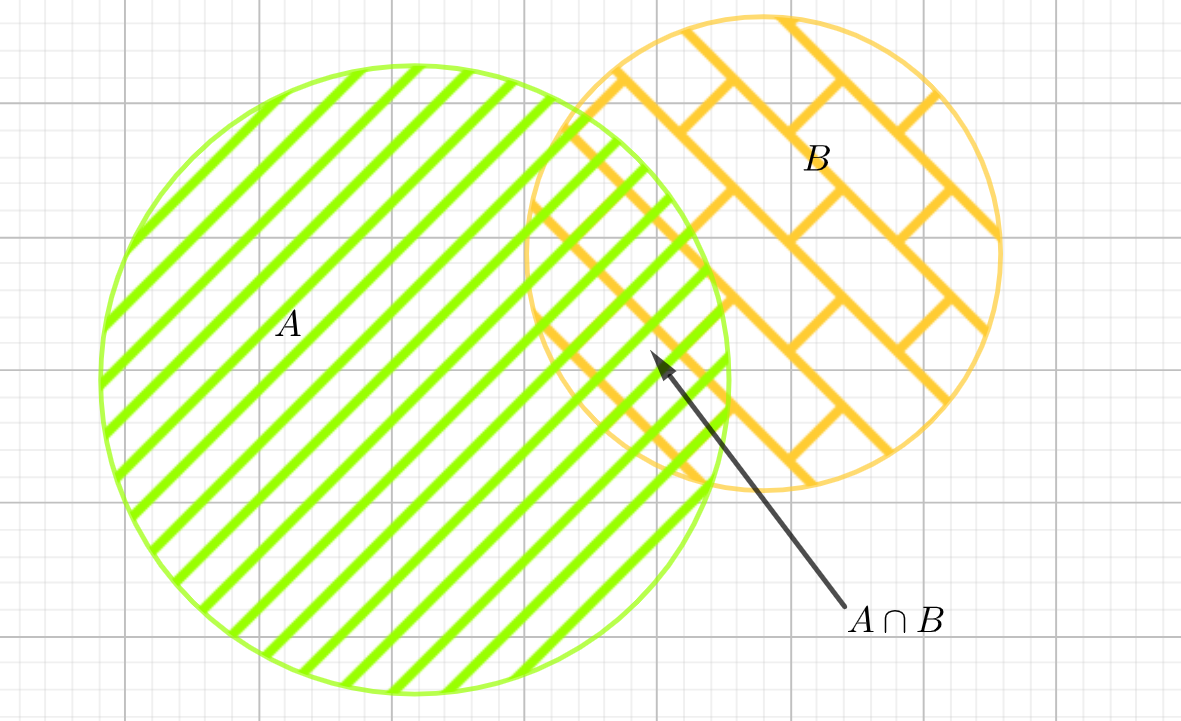
\includegraphics[scale=0.4]{cond_prob}}}
\hfill
\parbox[b][3 cm][t]{80mm}{
	Графически это означает, что, когда произошло событие $B$, мы оказались в круге $B$. 
	Тогда формула $$\frac{\Pro(AB)}{\Pro(B)}$$ есть просто вероятность попасть в $A\cap B$.
}

\newpage

Из определения следует так называемый <<Закон умножения вероятностей>>:
$$\Pro(A|B)\Pro(B)=\Pro(AB).$$

Легко проверяется, что $(B, \Ev_B, \Pro_B)$, где $\Ev_B = \Set{A \cap B}{A \in \Ev}$, 
так же является вероятностным пространством.

%\begin{Wtf}
%Зачем нужно требование $\Pro(B) > 0$, если можно в случае $\Pro(B) = 0$ доопределить 
%условную вероятность нулем как вероятность при условии невозможного события?
%При таком доопределении нарушится аксиома $3$. Вероятности $\Pro_B$, поскольку $\Pro_B(B)$ 
%по доопределению будет равно $0$.
%\end{Wtf}

\subsection{Независимость событий. Независимость в совокупности}

\qquad Да, и в теории вероятности есть независимость! Но это уже другая независимость, 
а не та, про которую так много новостей нынче.

\begin{Def}
События $A, B \in \Ev$ называются \mdef{независимыми}, если 
$$\Pro(AB) = \Pro(A) \Pro(B)$$.
\end{Def}

Для независимых событий $$\Pro(A|B) = \frac{\Pro(A)\Pro(B)}{\Pro(B)} = \Pro(A).$$

\begin{Ex}
Являются ли несовместные события ($A\cap B = \varnothing$) независимыми? 
Ответ: нет, пусть  $A, B \in \Ev \colon \Pro(A) > 0, \ \Pro(B) > 0$. 
Тогда $\Pro(AB) = \Pro(A)\Pro(B) = 0$, что является противоречием. По-простому, 
если произошло одно из несовместных событий, то второе уже не может произойти, 
и его условная вероятность равна $0$, а не вероятности самого события, 
что требуется для независимости.
\end{Ex}

Обобщим понятие независимости на произвольное количество событий.

\begin{Def}
События $A_1, A_2, \dots, A_n$ называются \mdef{независимыми в совокупности}, если 
$$\forall\, m = 2, \dots, n \quad \forall\, 1 \le j_1 < \ldots < j_m \le n \mapsto 
\Pro\left(\bigcap_{k=1}^{m}A_{j_k}\right)=\prod_{k=1}^{m} \Pro\left(A_{j_k}\right).$$
\end{Def}

\begin{Ex}
На примере тетраэдра Бернштейна можно убедиться в том, что попарной независимости 
событий недостаточно для независимости в совокупности. Рассмотрим тетраэдр, у 
которого три стороны покрашены в красный, синий и зеленый, а четвертая содержит все три цвета. 
События <<выпадет красный>> $=$ \{К\}, <<выпадет синий>> $=$ \{С\}, <<выпадет зеленый>> $=$ \{З\}
попарно независимы (например, вероятность события \{С\}$\cap$\{К\} равна вероятности 
выпадения четвертой грани, т. е. $1/4$, в то время как вероятность выпадения каждого цвета равна $1/2$). 
Однако $$\Pro(\{\text{С}\}\cap \{\text{К}\}\cap \{\text{З}\})=\frac14\neq\left(\frac12\right)^3.$$
\end{Ex}


\subsection{Формула полной вероятности. Формула Байеса}

\qquad Чуть выше мы рассмотрели условную вероятность, то есть поговорили о том, что
некоторые события могут пересекаться и когда в таких случаях можно сказать, что они
независимы. Часто встречается следующая группа событий.	
	
\begin{Def}
$B_1, \ldots, B_n$ образуют \mdef{полную группу}, если выполнены следующие условия:
	\begin{enumerate}
		\item $\Pro(B_i) > 0 \quad \forall i = 1, \ldots, n$,
		\item $B_iB_j = \varnothing \quad (i \not= j)$,
		\item $\bigcup\limits_{i=1}^nB_i = \Omega$.
	\end{enumerate}
\end{Def}

\begin{Th}
Пусть $B_1, \ldots, B_n$ образуют полную группу. Вероятность события $A \in \Ev$ можно 
вычислить по \emph{формуле полной вероятности}:
$$\Pro(A) = \sum\limits_{i=1}^{n} \Pro(A|B_i)\Pro(B_i)$$
\end{Th}

\begin{Proof}
$$A=\bigcup\limits_{i=1}^{n}AB_i, \quad AB_i \cap AB_j = \varnothing \quad (i \not= j),$$
$$\Pro(A) = \sum\limits_{i=1}^n \Pro(AB_i) = \sum\limits_{i=1}^{n} \Pro(A|B_i)\Pro(B_i).$$
Последний переход следует из  закона умножения вероятностей.
\end{Proof}

Первое требование определения полной группы необходимо для возможности определить 
условную вероятность, второе позволяет разбить множество $A$ на непересекающиеся части. 
Третье требование, вообще говоря, можно ослабить, потребовав, чтобы 
$A \subseteq \bigcup\limits_{i=1}^nB_i$. Доказательство при этом не изменится. \\

\begin{Ex}
Проиллюстрировать формулу полной вероятности можно обычным экзаменом: $A$ --- \{студент сдал экзамен\}, 
$B_i$ --- \{студент попал к преподавателю $i$\}. Как и в любой другой лотерее, можно оценить вероятность 
попадания к преподавателю $i$, то есть $\Pro(B_i)$, а трезво оценивая свои силы можно прикинуть 
и вероятность сдать тому или иному преподавателю $\Pro(A|B_i)$. Зная все вышеперечисленное, 
несложно по формуле вычислить вероятность успешной сдачи.
\end{Ex}

Формула полной вероятности используется для вычисления априорной вероятности, т.е. вероятности 
события, которое  еще не произошло. Пусть теперь $\Pro(A) > 0$. Тогда 
$\Pro(B_i|A)=\Pro(AB_i)/\Pro(A)$. Используя формулу полной вероятности, 
получаем \emph{формулу Байеса}:
$$\Pro(B_i|A)=\frac{\Pro(A|B_i)\Pro(B_i)}{\sum\limits_{j=1}^n\Pro(A|B_j)\Pro(B_j)}$$

Формула Байеса используется для вычисления апостериорной вероятности. То есть уже известно, что произошло некоторое событие $A$, и нужно вычислить вероятность
того, что произошло некоторое $B_i$. В примере с экзаменом, например, может быть известно, что студент не сдал экзамен, и хочется вычислить вероятность того, что он
сдавал преподавателю <<$P$>>.

\newpage
\end{document}
